\section{Introduction}
%architectural reviews,~\cite{guerreiro2014beyond}, large group chats ~\cite{mcnerney1999system}, data visualization~\cite{abbott2011empire}

While the primary use of virtual reality is in games and videos today, it can be used in numerous application domains, from education, architectural reviews, healthcare, large group chats, and data visualization, exploration of space and other dangerous locations, scientific visualization, manufacturing, journalism, traveling, architecture, and shopping.  

Virtual reality (VR) systems have become available to the general public recently and the virtual reality controllers introduced by HTC, Facebook, and Google have similar characteristics. 
Each includes a controller, shown in Figure~~\ref{fig:controllers}.
The Daydream controller, shown in Figure~\ref{fig:controllerDaydream}, in only for a single hand whereas the others have a controller for each hand.  The three major controllers all contain a way to track the thumb, at least 3 degrees of freedom tracking  (rotational), and at least four buttons.
Vive (\subref{fig:controllerVive}) and Oculus (\subref{fig:controllerOculus}) use an absolute tracking system to minimizing sensor drift and to allow for rotational and translational tracking~\cite{hilfert2016low}.  The Vive and Daydream (\subref{fig:controllerDaydream}) employ a thumb track pa!d to capture finger movement.  Oculus controller uses joysticks instead. 

\begin{figure}
  \centering
	\begin{subfigure}{.4\columnwidth}
  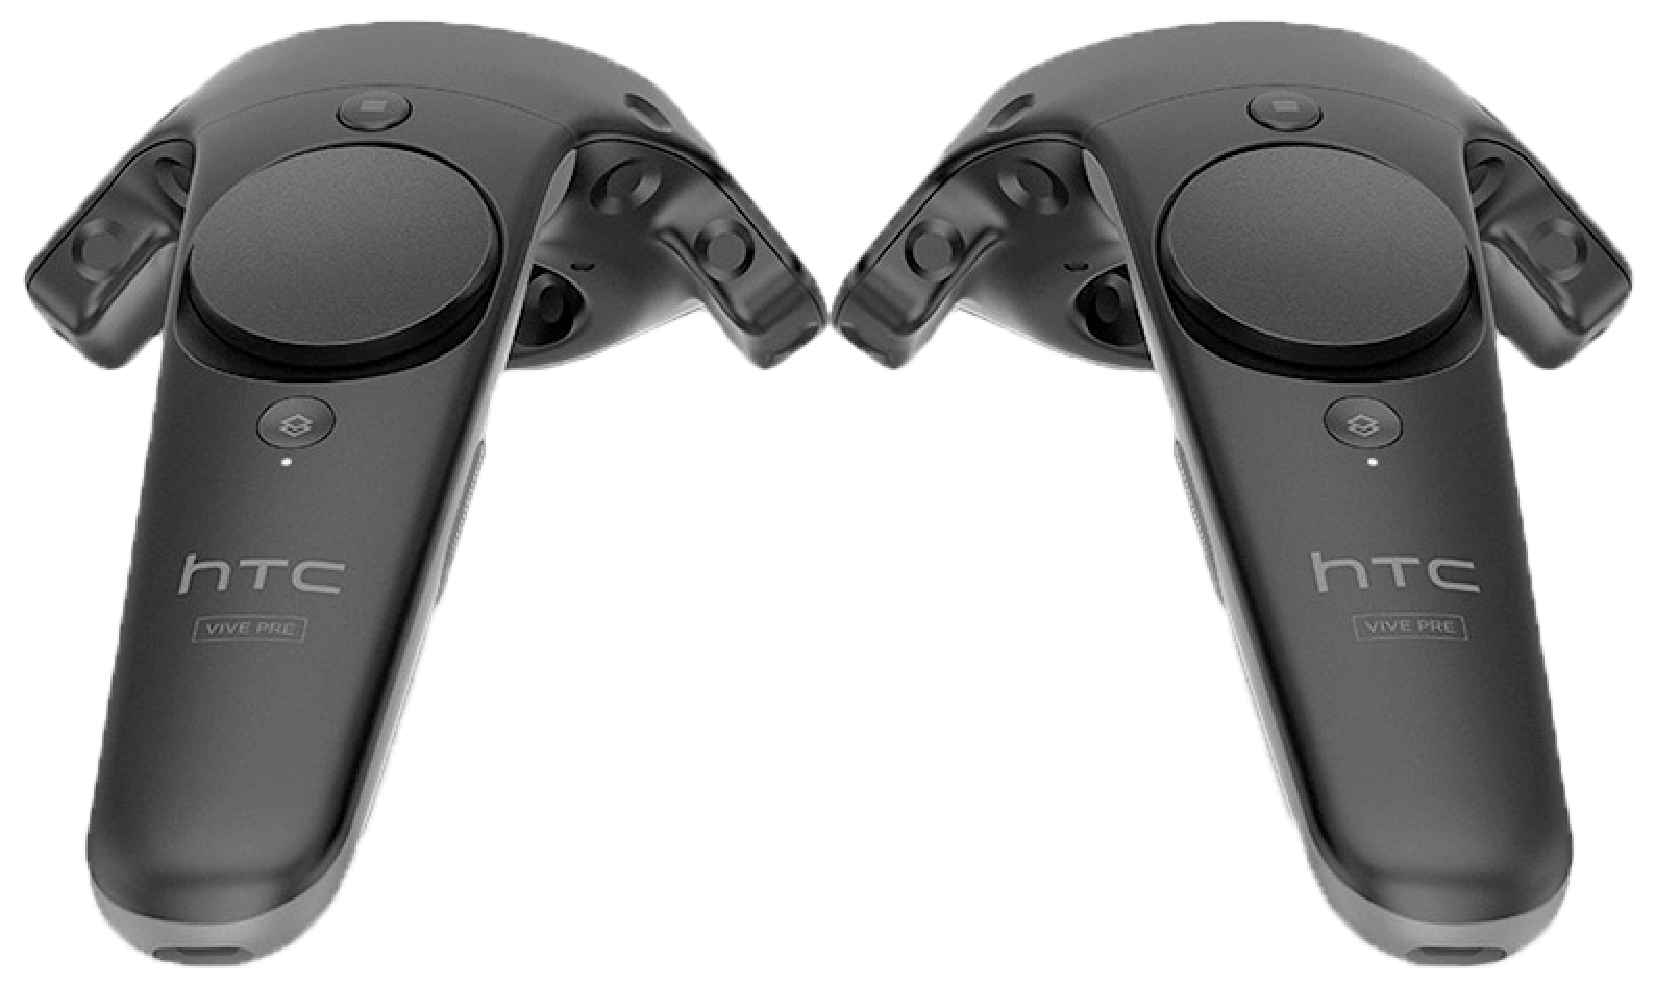
\includegraphics[width=\textwidth]{figures/controllerVive}
  \caption{HTC's Vive }\label{fig:controllerVive}
  \end{subfigure}
  \\
  \begin{subfigure}{.4\columnwidth}
  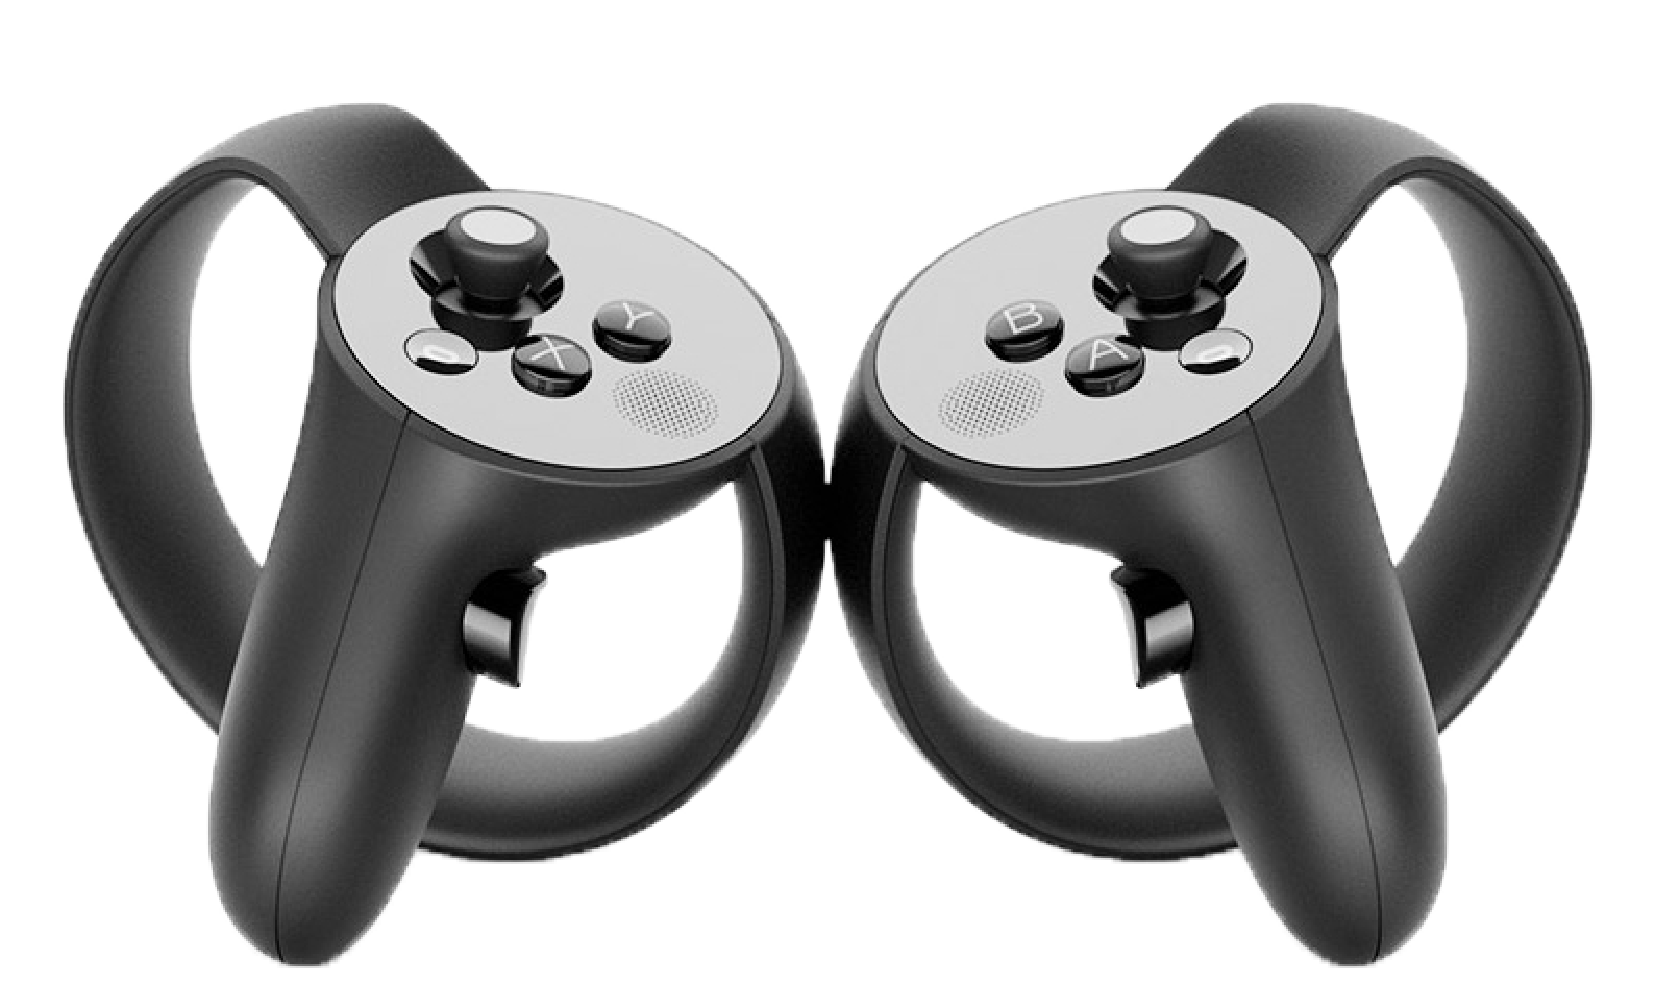
\includegraphics[width=\textwidth]{figures/controllerOculus}
  \caption{Facebook's Oculus}\label{fig:controllerOculus}
  \end{subfigure}
  \\
  \begin{subfigure}{.4\columnwidth}
  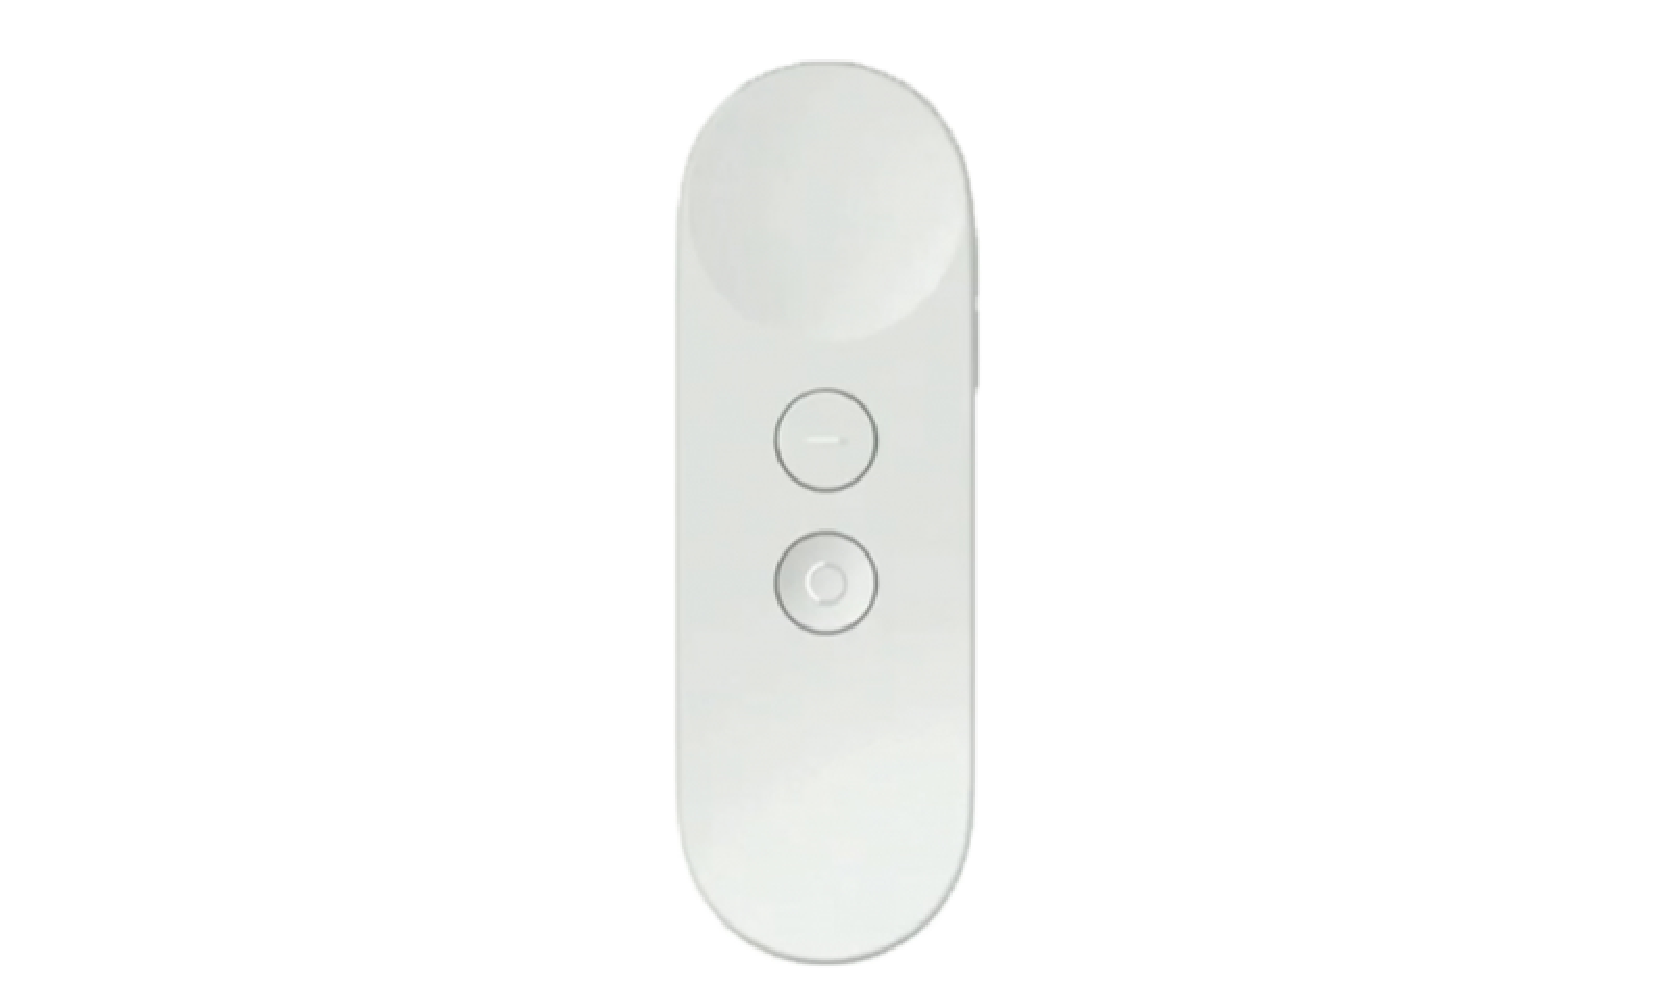
\includegraphics[width=\textwidth]{figures/controllerDaydream}
  \caption{Google's Daydream}\label{fig:controllerDaydream}
  \end{subfigure}
  \caption{Virtual reality controllers}
~\label{fig:controllers}

\end{figure}

Even though typing is not prevalent in immersive virtual reality, text entry is still important, with a wide range of uses: from typing in account names and passwords, searching items, specifying parameters used in the applications, referring to friends,  writing notes and chatting with others, etc.      

The average typing performance on a regular keyboard was found to be about 60 words per minute\cite{varcholik:textentry}, thanks to the dexterity of our fingers, the haptic feedback from the physical keyboards, and visual feedback on the display.    In the context of virtual reality, it is often not an option to use a physical keyboard.  We are usually not sitting down and it is hard to switch between the VR controllers and a physical keyboard, further complicated by the fact that we cannot see the keyboard in VR.  To avoid having to remove the head gear to type, it is desirable to enter text using existing VR controllers. 

Typing is challenging in virtual reality because of the latency in visual feedback and the lack of proprioception.  The industry standard is to enter text with gaze.  A virtual keyboard is presented in VR, and users type a letter by gazing at the desired key and tapping on the controller.   It was found that the users can typically type at about 7 words per minute.   Entering text via speech is attractive, especially in the immersive virtual reality environment.  Speech may not be suitable when entering names and URLs, especially in public spaces due to privacy issues.  Furthermore, speech often needs to be corrected via text editing.  Other alternatives proposed including using gesture, motion controllers, Leap Motion or tangibles, handheld controllers, or relying on a subset of keyboard and mouse commands~\cite{billinghurst1999collaborative}.
All these existing solutions, while potentially good for simple tasks, aren't adequate for tasks that requires a greater bandwidth of input~\cite{McGill:2015:DRO:2702123.2702382}.



\subsection{Methodology}

The goal of the paper is to understand how we can enter text simply, quickly, and accurately via the touchpad found in commodity VR controllers today.  
\begin{enumerate}
\item
We started our investigation by exploring existing ideas.  The ideas we explored include   
\begin{enumerate}
\item
Gazing.  Users enter keys by gazing at the keys in a virtual keyboard. 

\item
Drumming.  Keys are displayed as a virtual drum kit, users enter keys by hitting the corresponding drums using the controllers as drumsticks\cite{Google:VRdrum}. 

\item
Augmented reality.  A camera is used to stream the view of the touchpad and fingers into
virtual reality.  

\item
26-key tapping.  Users use the touchpad to tap on the virtual keyboard displayed in the VR. 

\item
26-key swiping.  Users use the touchpad to swipe on the virtual keyboard displayed in the VR. 
\end{enumerate}
We built a prototype of each of these systems and tested it informally on a couple of users.  This study revealed major deficiencies in each of these approaches.  

\item
We propose a new virtual keyboard, Slide, that incorporates the learning from our initial investigation.  It is based on three main design concepts: 
\begin{enumerate}
\item
Relative vectors.  To enter a character, the user slides from what is assumed to be the center of the keyboard to the key of interest.  

\item
Directional input, with error correction.  All keys are grouped in 6 tiles, and the user only has to slide in the direction of the tile containing the key.  A Bayesian word recommender determines the word entered. 

\item
Intention-based hybrid keyboard: the keyboard automatically switches between the 26-key and 6-tile keyboard based on the user's finger movements.  
\end{enumerate}

\item 
We implemented the proposed technique in the Vive system; note that Slide is applicable to the other VR controllers as well.   We conducted a study with 15 users and evaluated the speed, accuracy, as well as the learnability of the system. 
\end{enumerate}

\subsection{Contribution}
This paper proposes Slide, a VR text entry technique that requires only a touch pad.  To address the visual latency and lack of proprioception in VR, we have adopted relative positioning with a heavy use of auto-correction.  The virtual keyboard is divided into six tiles placed around the center of the keyboard.  The user needs to slide his finger in one of the six directions towards the tile containing the character, and error correction is used to pick the most likely word.  Our study shows that users can type at the speed of 34 words per minute on average, with an error rate of 4\%.   

Slide allows for graceful degradation, when better control over the text entry is necessary, such as for typing in passwords.  The user can fall back to sliding to the precise key; our keyboard automatically detects the use of the more precise mode by observing the speed of the sliding motion.  The users can type at about 12 words per minute using this slow but more precise entry method.


